%!TEX root = /Users/stevenmartell/Documents/CONSULTING/HumpbackChub/HBC_2011_Assessment/WRITEUP/HBCmain.tex
\section{Methods} % (fold)
\label{sec:methods}

There are two major methodological components in this length-based model: (1) the development of an individual based model (IBM) for simulating a capture recapture program, and (2) a statistical catch-at-length mark-recapture model to estimate the number of individual fish in each length-class in each sampling year.  A detailed description of the IBM simulation model is provided in the appendix; in short, this simulation model generates a matrix of the number of fish captured-at-length, a matrix of the number of newly marked fish released-at-length, and a matrix of marked fish recaptured-at-length.  The remained of this section is a detailed analytical description of the statistical catch-at-length model used to estimate the abundance-at-length of humpback chub in the Grand Canyon.

The following is a description of the analytical model for the length-structured mark-recapture model (hereafter, LSMR) used in this assessment.  I present the analytical model in the form of a table where the order in which model equations are presented also represent the order in which the calculations proceed in the computer code.  Equations presented in each table are referenced, for example, as \eqref{eq:T1.1}, where the T1 refers to Table \ref{table:LSMRmodel}, and the .1 refers to the first equation in that table. The LSMR model was implemented in AD Model Builder \citep{fournier2011ad}, and the template code is available in the appendix of this document as well as a Git code repository (\url{https://code.google.com/p/lsmr-project/}).  The description of the Length-Structured Mark-Recapture (LSMR) model is broken down into: input data, estimated parameters, dynamics of numbers-at-length, capture probability, and negative log-likelihoods and prior densities.

The following notation is used to define the dimensions of various variables. Vector quantities are designated with an an arrow ($\vec{x}$) or with a single subscript, and matrix is denoted by boldface uppercase letters ($\mathbf{X}$) and where two subscripts are shown denotes the element specific calculation.  Higher dimensional arrays are indicated by normal upper case letters with 3 or more subscripts.  

\subsection{Input data} % (fold)
\label{sub:input_data}

The model dimensions consists of time intervals (year indexed by $i$) and length intervals (index by $j$, \ref{eq:T1.1}).  Capture-recapture data for the humpback chub have been collected on an annual basis since May 1, 1989,  and the latest capture record in this analysis is February 27, 2012.  The principle input data for LSMR consists of model dimensions (e.g., years, length intervals), catch-at-length $\mathbf{C}_{ij}$ for each year, the number of new marks released at length $\mathbf{M}_{ij}$, and the number of recaptured marks at length $\mathbf{R}_{ij}$.


% subsection input_data (end)

\subsection{Estimated parameters \& parametric functions} % (fold)
\label{sub:estimated_parameters}
An array of estimated parameters is denoted by $\Theta$ and consists of 8 +$(I-1)$ +$J$ unknowns where $I$ is the total number of years and $J$ is the total number of length intervals.  The average initial numbers-at-length is defined as $\dot{N}$, and the average number of new recruits at each time step is denoted by $\bar{R}$.  To initialize the number of individuals in each length interval $\Lambda$ in the initial year $i=1$, the average initial number is multiplied by a length specific lognormal deviate $\eta_j$ \eqref{eq:T1.11} with the added constraint $\sum_j \eta_j = 0$ to ensure that $\dot{N}$ is identifiable. Similarly, the average number of newly recruiting fish in each time step is based on deviates at each time-step from the mean recruitment \eqref{eq:T1.12}, where again the constraint $\sum_i \nu_i = 0$ ensures that $\bar{R}$ is identifiable.

Natural mortality is a function of length \eqref{eq:T1.6}, where the natural mortality at the asymptotic length $M_\infty$ is estimated from the data. Selectivity is also assumed to be a parametric function of length \eqref{eq:T1.7} where $l_x$ and $g_x$ represent length-at-50\% vulnerability and the standard deviation of the logistic function, respectively.  Note that in \eqref{eq:T1.6} the estimated natural mortality rate is confounded with asymptotic length $l_\infty$ which is also an estimated parameter along with the von Bertalanffy growth coefficient $k$.  The growth parameters are used to calculate a vector of growth increment $\vec{\Delta}$ assuming von Bertalanffy growth \eqref{eq:T1.8}. An additional parameter $\beta$ is used to characterize the variability in annual growth increments for individual fish. 

\subsection{Growth transition} % (fold)
\label{sub:growth_transition}
The asymptotic length $l_\infty$ is defined as the average asymptotic length for a population of fish.  It is assumed in \eqref{eq:T1.8} that individuals greater than $l_\infty$ continue to grow at a much reduced rate $k$; this is accomplished by exponentiating the growth increment equation ($(l_\infty-x_j)(1-exp(-k\tau))$), adding 1.0, and taking the natural logarithm ensuring that \eqref{eq:T1.8} remains positive for all positive values of $l_\infty$, $k$, and $\Lambda$.
The probability of transitioning from one length interval $x_j$ to length intervals greater than $x_{j}$ is based on a gamma density function \eqref{eq:T1.9}, where the mean is denoted by $\Delta_j$ and a variance equal to $\Delta_j \beta$.  Each row of $\mathbf{P}_{j,j'}$ is normalized to sum to 1.0, and $\mathbf{P}_{j,j'}=1.0$ when $j=j'=n$, where $n$ is the number of length intervals (i.e., individuals in the last length interval represent a plus group).



% subsection growth_transition (end)


% subsection estimated_parameters (end)

\subsection{Dynamics of numbers-at-length} % (fold)
\label{sub:dynamics_of_numbers_at_length}

% subsection dynamics_of_numbers_at_length (end)

\subsection{Length-based capture probability} % (fold)
\label{sub:length_based_capture_probability}

% subsection length_based_capture_probability (end)

\subsection{Negative log-likelihoods and prior densities} % (fold)
\label{sub:negative_log_likelihoods_and_prior_densities}

% subsection negative_log_likelihoods_and_prior_densities (end)

\subsection{Length-structured mark-recapture model (LSMR)}






\begin{table}
  \centering
\caption{Data, parameters, and analytical procedures for the length-based mark-recapture model.}\label{table:LSMRmodel} 
\tableEq
	\begin{small}
    \begin{align}
        \hline
		&\mbox{INDEXES, DATA \& CONSTANTS} \nonumber\\
		&\mbox{index for time, index for length interval} 
		&i,j \label{eq:T1.1}\\ 
		&\mbox{time step}  & \tau\\
		&\mbox{set of midpoints of length intervals}
		&\Lambda = \{x_1, \ldots,x_J\}\\
		&\mbox{catch, new marks, recaptures} 
		&\mathbf{C}_{i,j}, \mathbf{M}_{i,j}, \mathbf{R}_{i,j}\\[1ex]
		%%
		%%
		&\mbox{PARAMETERS \& DERIVED VARIABLES} \nonumber\\
		&\mbox{estimated parameters} 
		&\Theta=\{\dot{N},\bar{R},M_\infty,l_\infty,k,\beta,l_x,g_x,
			\vec{\eta},\vec{\nu} \}\\
		&\mbox{mortality-at-length} 
		& \vec{m} = \frac{M_\infty l_\infty}{\Lambda}
		\label{eq:T1.6}\\
		&\mbox{selectivity-at-length} 
		& \vec{s} = \frac{1}{1+\exp(-(\Lambda-l_x)/g_x)}
		\label{eq:T1.7}\\
		&\mbox{growth increment} 
		& \vec{\Delta} = \ln( \exp[(l_\infty-\Lambda)(1-\exp(-k \tau))] +1)
		\label{eq:T1.8}\\
		&\mbox{length transition probability}
		& \mathbf{P}_{j,j'} =\int_{x_j-x^*}^{x_j+x^*} \frac{x_{j'}^{(\Delta_{j}/\beta-1)}
		e^{x_{j'}/\beta}}{\beta^{\Delta_{j}/\beta} \Gamma(\Delta_{j}/\beta)}dx, \nonumber\\
		& &\quad \sum_{j'=1}^J P_{j,j'}= 1 
		\label{eq:T1.9}\\
		&\mbox{total numbers, marked numbers} 
		& \mathbf{N}, \mathbf{T}\\[1ex]
		%%
		%%
		&\mbox{INITIAL STATES ($i=1$, $j=1$)}  \nonumber\\
		&\mbox{initial numbers-at-length}
		&\mathbf{N}_{i,j} = \dot{N}\exp(\eta_j), \quad \mbox{where} \sum_j \eta_j=0
		\label{eq:T1.11}\\
		&\mbox{new recruits}
		&\mathbf{N}_{i,j} = \bar{R}\exp(\nu_i), \quad \mbox{where} \sum_i \nu_i=0
		\label{eq:T1.12}\\
		%%
		%%
		&\mbox{DYNAMIC STATES ($i>1$)} \nonumber\\
		&\mbox{capture probability} 
		& f_i\\
		\hline \nonumber
    \end{align}
\end{small}
    \normalEq
\end{table}

% section methods (end)

\begin{figure}[htbp]
	\centering
		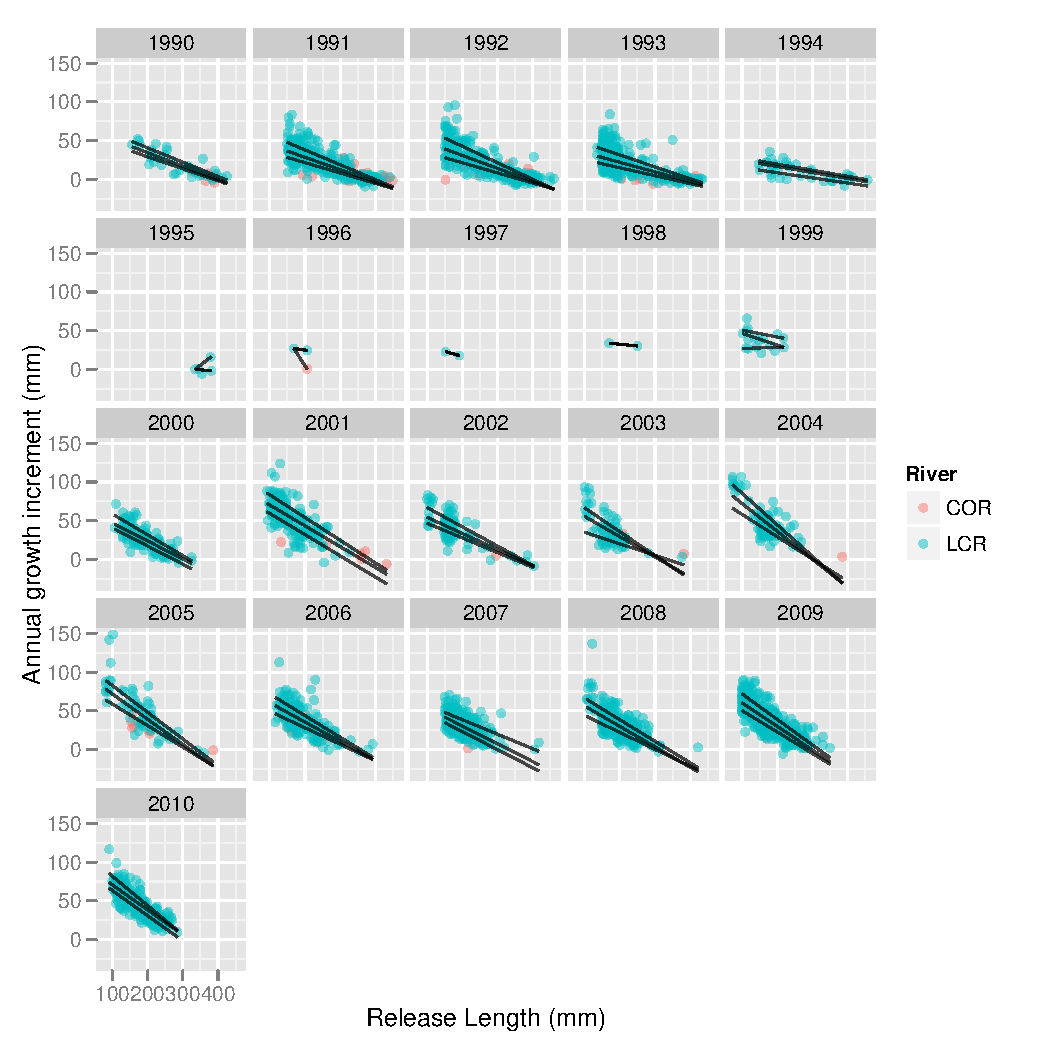
\includegraphics[height=4in]{../FIGS/LSMR/fig:GrowthIncrements.pdf}
	\caption{caption}
	\label{fig:FIGS_LSMR_fig:GrowthIncrements}
\end{figure}

